\section{Experiments}
\subsection{Tpch SF10}
\subsubsection{Memory footpring error}
\begin{figure}[ht]
  \centering
  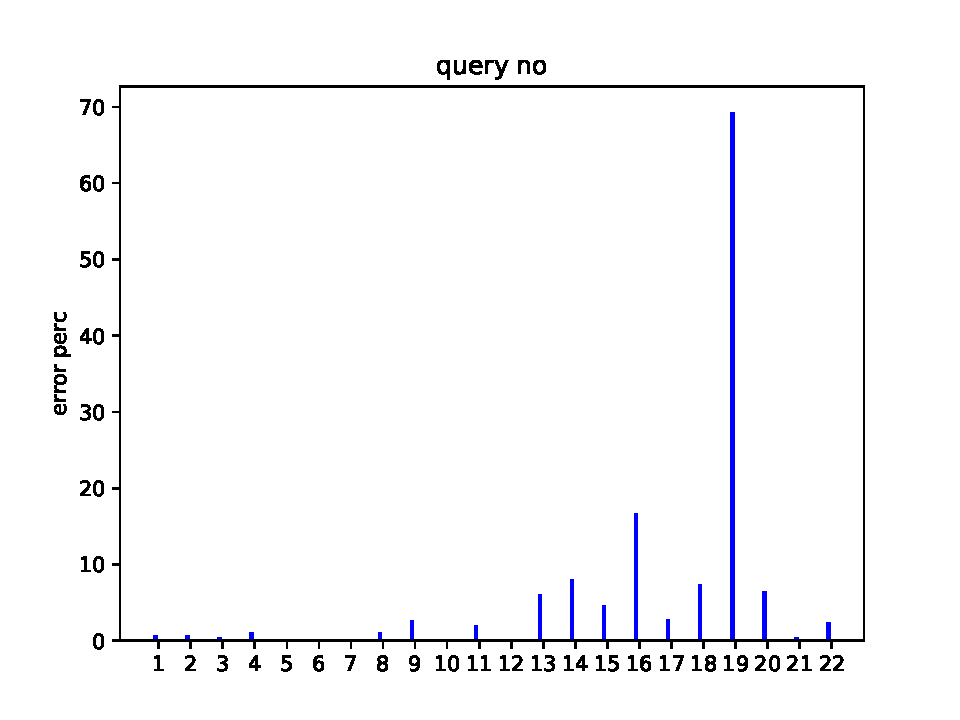
\includegraphics[scale=0.7]{figs/tpch10/mem_error_1-23.pdf}
  \caption{Queries 1-22 memory footprint error}
  \label{fig:tpch10m}
\end{figure}

% \subsection{Select Error for tpch-sf-10}
%
% \subsection{Whole query evaluation}
%

\subsection{Airtraffic Queries}
\subsubsection{Q04}

\begin{figure}[t]
\begin{lstlisting}
SELECT "DayOfWeek", COUNT(*) AS "Flights"
FROM ontime
WHERE "DepDelay" > 15
GROUP BY "DayOfWeek"
ORDER BY "DayOfWeek";
\end{lstlisting}
  \caption{Query 4}
  \label{sel:sql4}
\end{figure}
Randomization point: DepDelay

\begin{figure}[t!]
  \begin{subfigure}[t]{0.5\textwidth}
    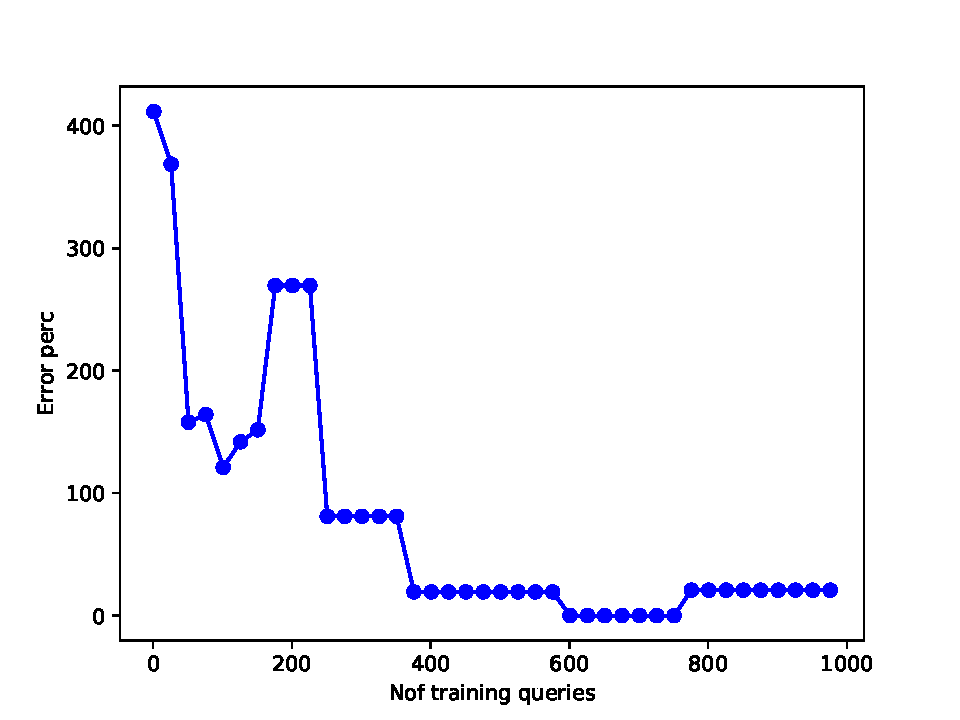
\includegraphics[scale=0.4]{figs/airtraffic/airtraffic_sel04_error.pdf}
    \caption{Query 04 select error}
    \label{fig:sel19}
  \end{subfigure}
  \begin{subfigure}[t]{0.5\textwidth}
    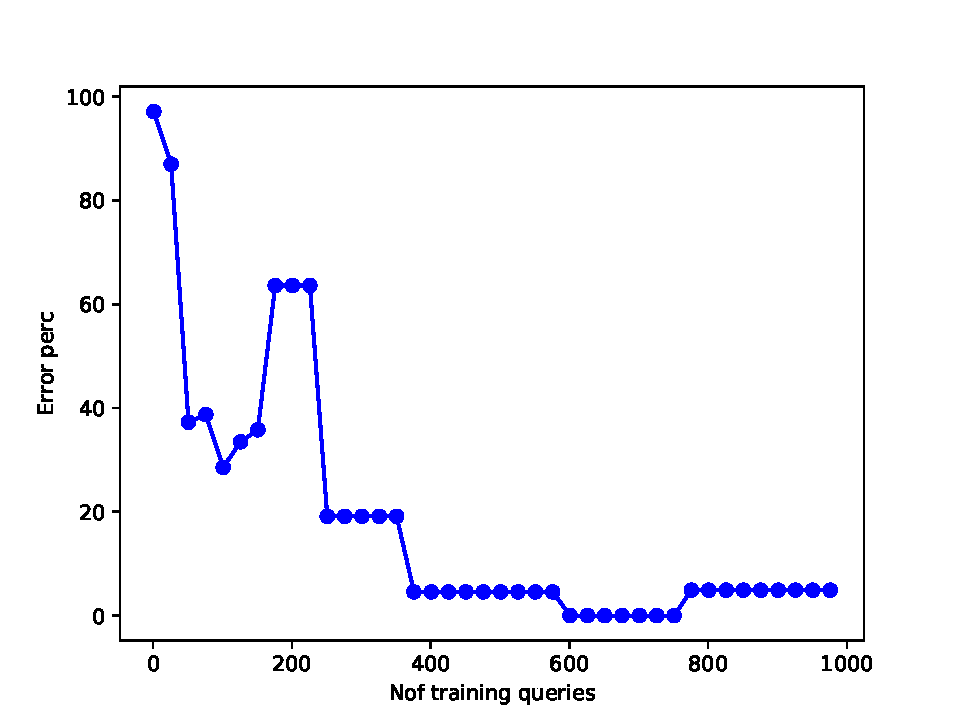
\includegraphics[scale=0.4]{figs/airtraffic/airtraffic_q04_memerror.pdf}
    \caption{Query 04 memory footprint}
    \label{fig:sel19}
   \end{subfigure}
\end{figure}

\subsubsection{Q09}

\begin{figure}[t]
\begin{lstlisting}[frame=single]
WITH t1 AS (
    SELECT "Origin", "CRSDepTime", "DepDelay", "Dest", "ArrDelay", "CRSArrTime"
    FROM ontime
    WHERE "DepDelay" > 15 AND "ArrDelay" > 15
      AND "Month" = 3 AND "DayofMonth" = 24 AND "Year" = 2013
)
SELECT t1."Origin" AS "Airport1",
       CAST(AVG(t1."DepDelay") AS DECIMAL(8,2)) AS "AVGDepDelay",
       CAST(AVG(t1."ArrDelay") AS DECIMAL(8,2)) AS "AVGArrDelay", t2."Origin" AS "Airport2",
       CAST(AVG(t2."DepDelay") AS DECIMAL(8,2)) AS "AVGDepDelay2",
       CAST(AVG(t2."ArrDelay") AS DECIMAL(8,2)) AS "AVGArrDelay2", t2."Dest" AS "Airport3"
FROM t1, t1 AS t2
WHERE t1."Dest" = t2."Origin" AND t1."CRSArrTime" < t2."CRSDepTime"
GROUP BY t1."Origin", t2."Origin", t2."Dest"
ORDER BY "AVGDepDelay" DESC, "AVGArrDelay" DESC, "AVGDepDelay2" DESC, "AVGArrDelay2" DESC
\end{lstlisting}
  \caption{Query 09}
  \label{sel:sql09}
\end{figure}

\begin{figure}[t!]
  \begin{subfigure}[t]{0.5\textwidth}
    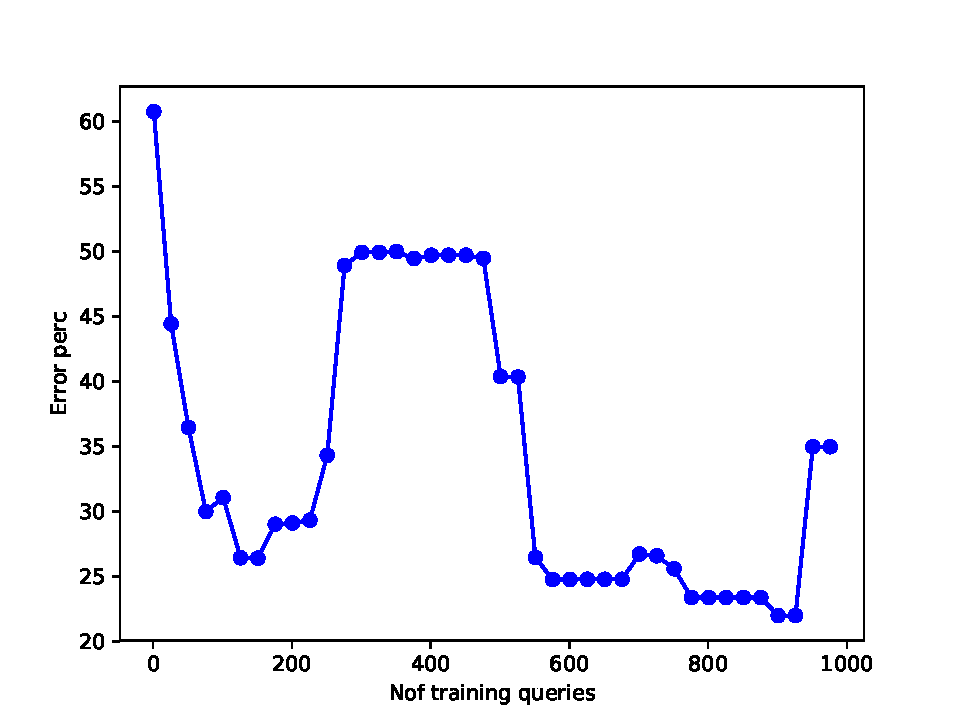
\includegraphics[scale=0.4]{figs/airtraffic/airtraffic_sel09_error.pdf}
    \caption{Query 09 select error}
    \label{fig:sel19}
  \end{subfigure}
  \begin{subfigure}[t]{0.5\textwidth}
    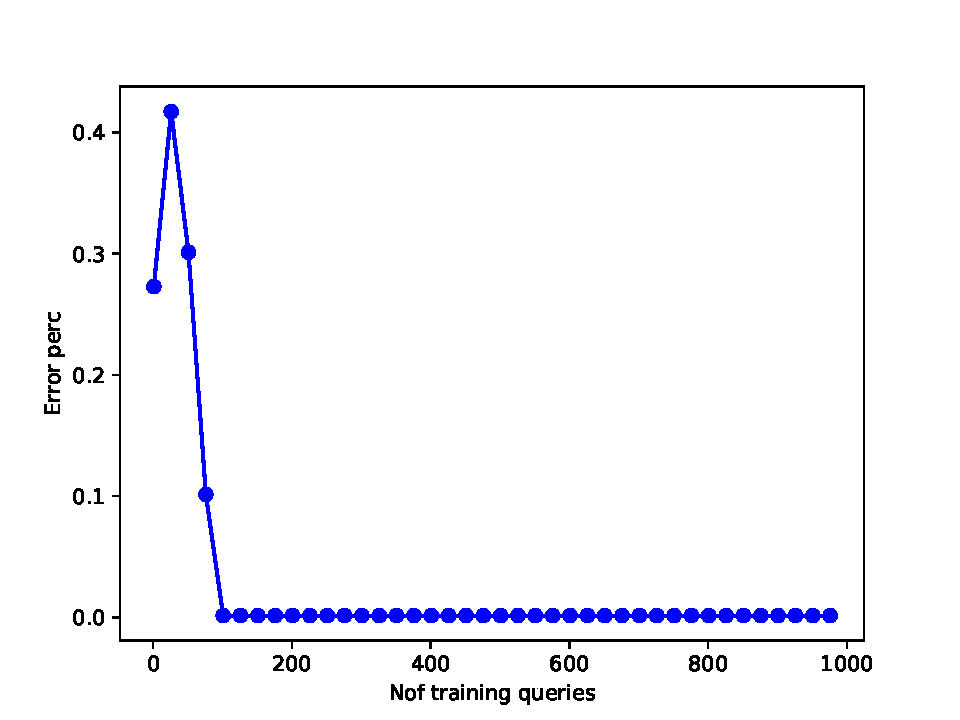
\includegraphics[scale=0.4]{figs/airtraffic/airtraffic_q09_memerror.pdf}
    \caption{Query 09 memory footprint}
    \label{fig:sel19}
   \end{subfigure}
\end{figure}

\subsubsection{Q11}

\begin{figure}[t]
\begin{lstlisting}[frame=single]
WITH t1 AS ( -- #flights per route before 9/11
    SELECT SQL_MIN("Origin", "Dest") || ' <-> ' ||
           SQL_MAX("Origin", "Dest") AS route,
           COUNT(*) AS cnt_before
    FROM ontime
    WHERE '2010-09-11' < "FlightDate" AND "FlightDate" < '2011-09-11'
    GROUP BY route
),
t2 AS ( -- #flights per route after 8/11
    SELECT SQL_MIN("Origin", "Dest") || ' <-> ' ||
           SQL_MAX("Origin", "Dest") AS route,
           COUNT(*) AS cnt_after
    FROM ontime
    WHERE '2011-09-11' <= "FlightDate" AND "FlightDate" < '2012-09-11'
    GROUP BY route
),
t3 AS ( -- merge t1, t2 into one table
    SELECT t1.route AS route1, t1.cnt_before, t2.route AS route2, t2.cnt_after
    FROM t1 FULL OUTER JOIN t2 ON (t1.route = t2.route)
)
SELECT CASE WHEN route1 IS NULL THEN route2 ELSE route1 END AS "Route",
       cnt_before AS "FlightsBefore", cnt_after AS "FlightsAfter"
FROM t3;
\end{lstlisting}
  \caption{Query 11}
  \label{sel:sql11}
\end{figure}

\begin{figure}[t!]
 \begin{subfigure}[t]{0.5\textwidth}
   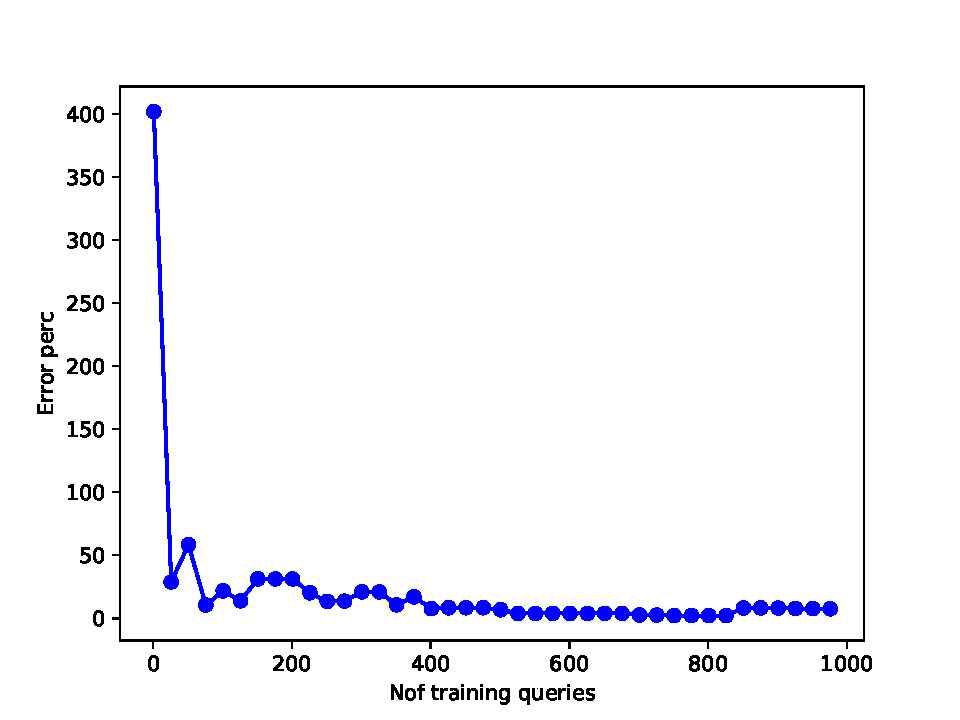
\includegraphics[scale=0.4]{figs/airtraffic/airtraffic_sel11_error.pdf}
   \caption{Query 11 select error}
   \label{fig:sel11}
 \end{subfigure}
 \begin{subfigure}[t]{0.5\textwidth}
   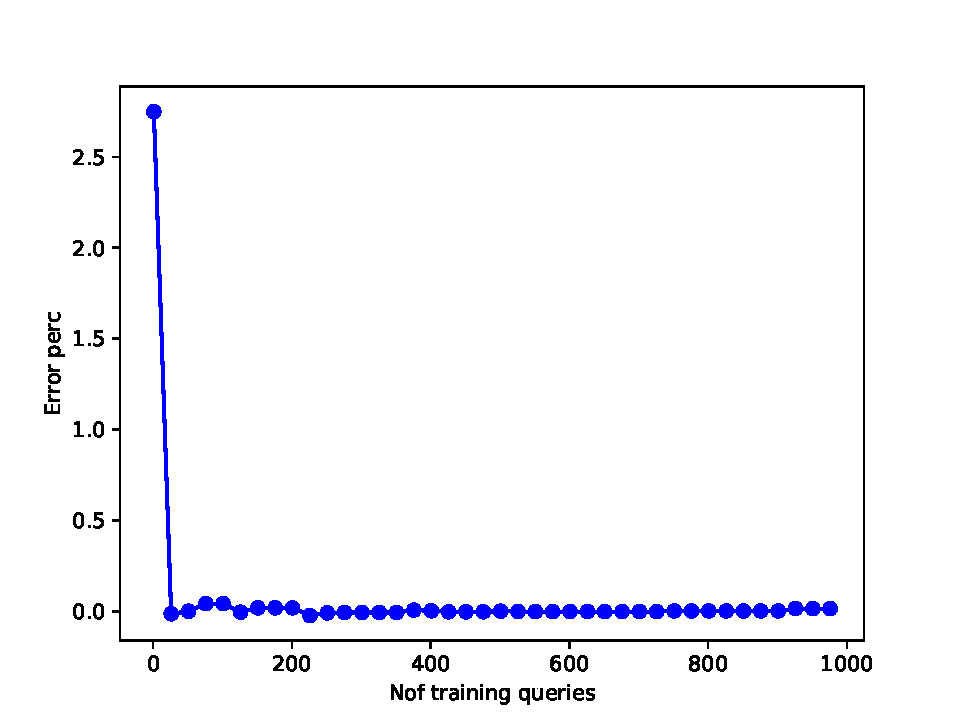
\includegraphics[scale=0.4]{figs/airtraffic/airtraffic_q11_memerror.pdf}
   \caption{Query 11 memory footprint}
   \label{fig:sel11}
  \end{subfigure}


\end{figure}


\subsubsection{Q15}

\begin{figure}[t]
\begin{lstlisting}[frame=single]
WITH t1 AS (
    SELECT "Carrier", CAST (FLOOR("CRSDepTime"%2400/100) AS INT) AS "Hour",
           CAST(AVG("ArrDelay") AS DECIMAL(8,2)) AS "PredictedArrDelay"
    FROM ontime
    WHERE "Year" = 2007 AND "Month" = 10 AND "DayofMonth" = 24
    GROUP BY "Carrier", "Hour"
),
t2 AS (
    SELECT t."Carrier", tmp.*
    FROM tmp, (SELECT DISTINCT "Carrier" FROM t1) AS t
)
SELECT "Carrier", "Hour", SUM("PredictedArrDelay")
FROM (SELECT * FROM t1 UNION SELECT * FROM t2) AS t
GROUP BY "Carrier", "Hour"
ORDER BY "Carrier", "Hour";
\end{lstlisting}
  \caption{Query 15}
  \label{sel:sql15}
\end{figure}


\begin{figure}[t!]
  \begin{subfigure}[t]{0.5\textwidth}
    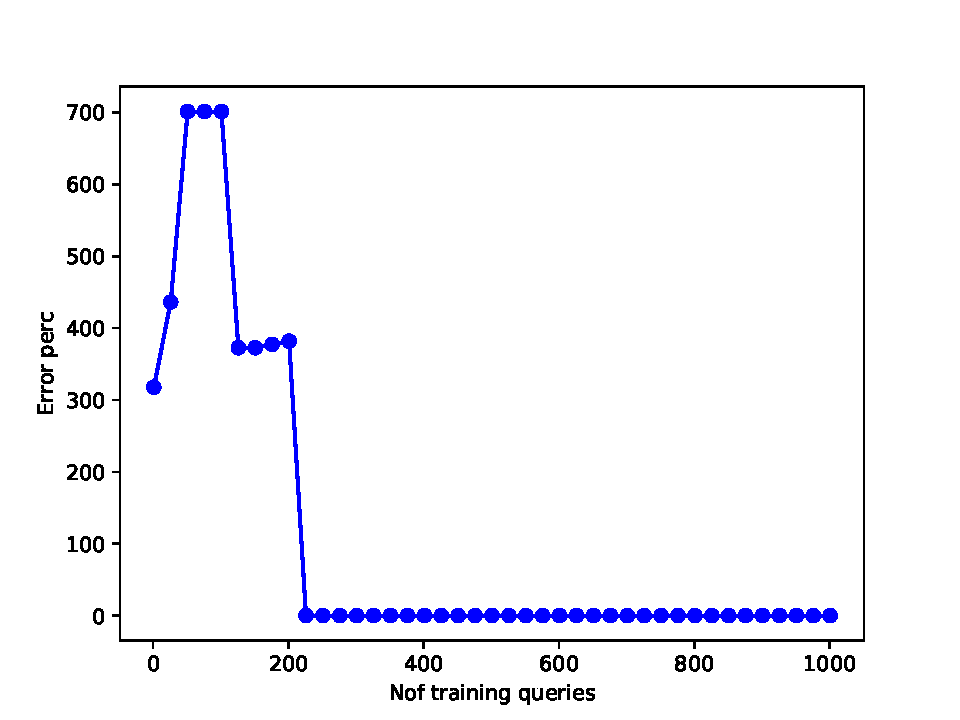
\includegraphics[scale=0.4]{figs/airtraffic/airtraffic_sel15_1_error.pdf}
    \caption{Query 15 select error}
    \label{fig:sel19}
  \end{subfigure}
  \begin{subfigure}[t]{0.5\textwidth}
    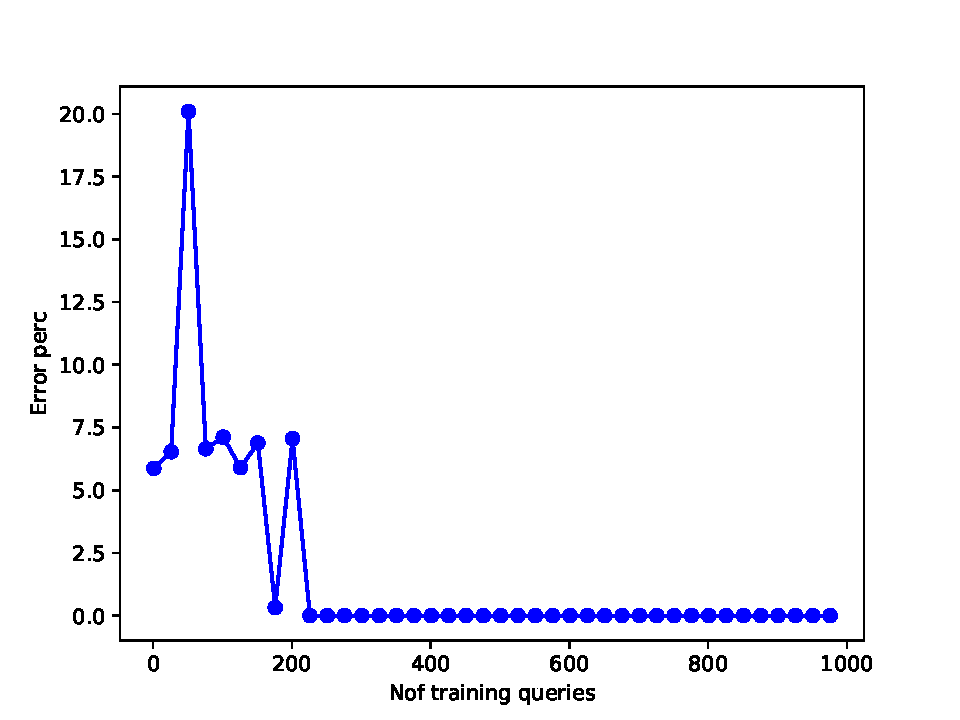
\includegraphics[scale=0.4]{figs/airtraffic/airtraffic_q15_1_memerror.pdf}
    \caption{Query 15 memory footprint}
    \label{fig:sel19}
   \end{subfigure}

\end{figure}

\subsubsection{Q19}

\begin{figure}[t]
\begin{lstlisting}[frame=single]
SELECT CAST (FLOOR("CRSDepTime"%2400/100) AS INT) AS "Hour",
       "Origin", "Dest", "Carrier",
       CAST(SUM("DepDel15") AS DOUBLE)/COUNT(*) >= 0.5 AS "PossibleLongDelay"
FROM ontime
GROUP BY "Origin", "Dest", "Carrier", "Hour"
ORDER BY "PossibleLongDelay", "Hour", "Origin", "Dest", "Carrier";
\end{lstlisting}
  \caption{Query 19}
  \label{sel:sql19}
\end{figure}


\begin{figure}[t!]
  \begin{subfigure}[t]{0.5\textwidth}
    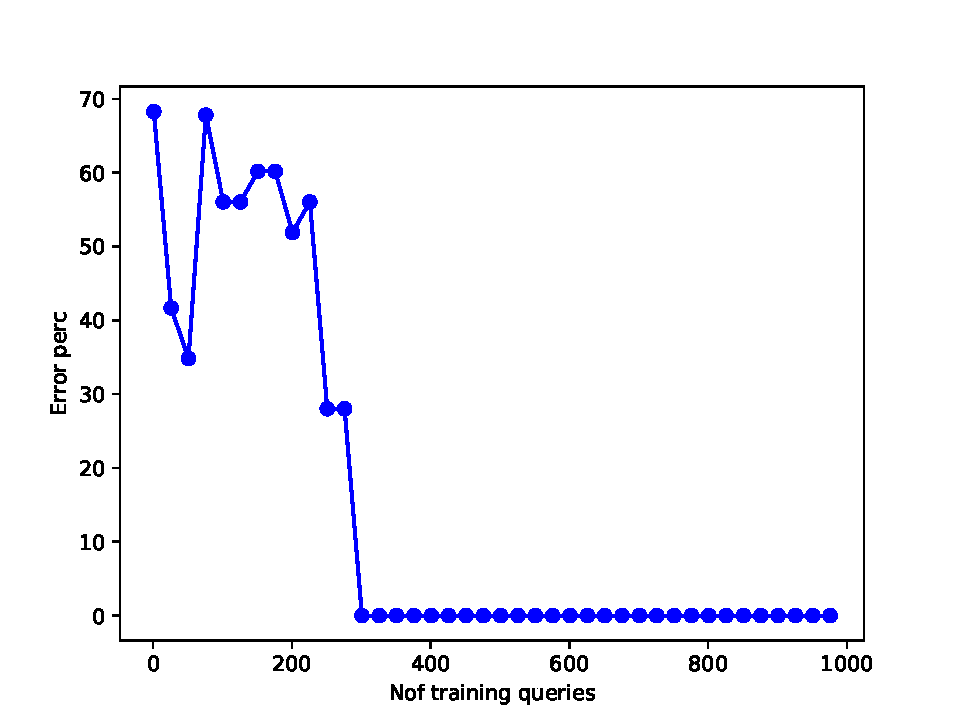
\includegraphics[scale=0.4]{figs/airtraffic/airtraffic_sel19_1_error.pdf}
    \caption{Query 19 select error}
    \label{fig:sel19}
  \end{subfigure}
  \begin{subfigure}[t]{0.5\textwidth}
    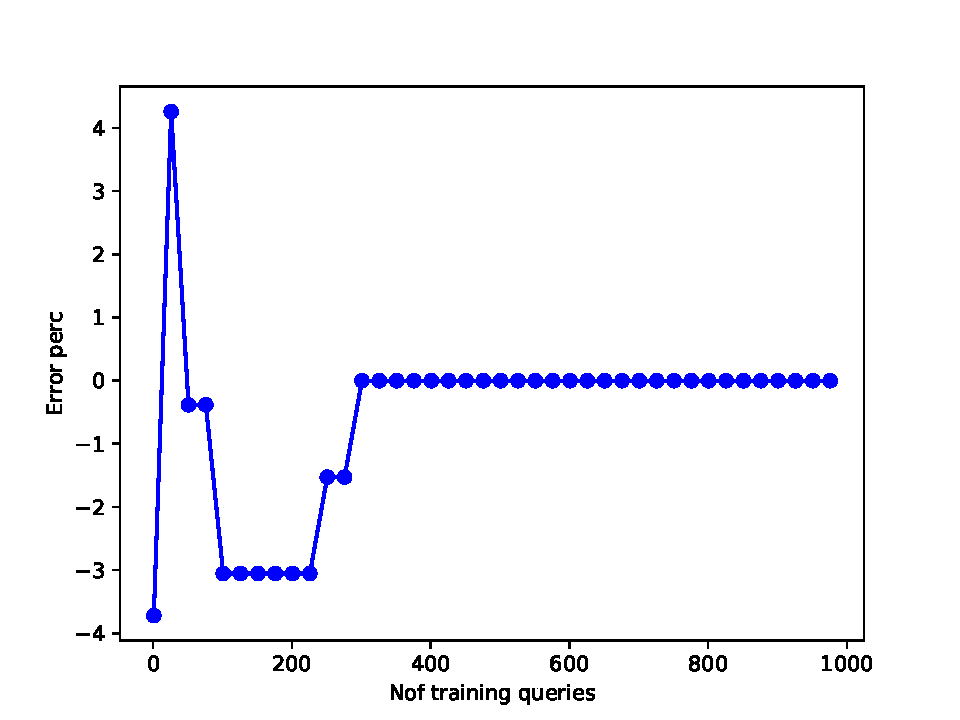
\includegraphics[scale=0.4]{figs/airtraffic/airtraffic_q19_1_memerror.pdf}
    \caption{Query 19 memory footprint}
    \label{fig:sel19}
   \end{subfigure}

\end{figure}



% \begin{figure}[ht]
%   \centering
%   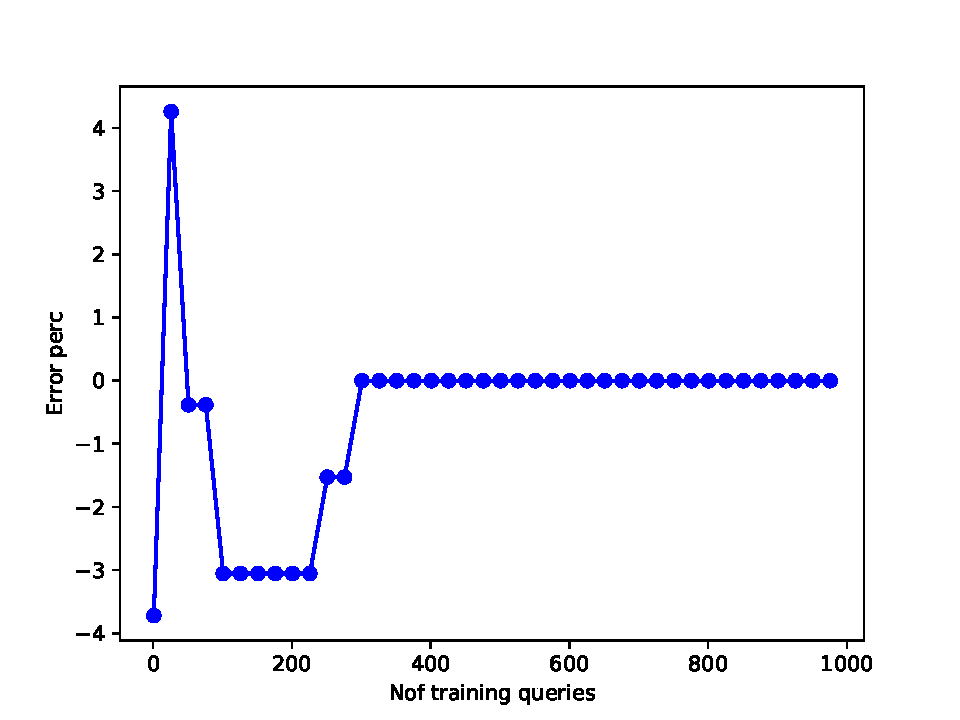
\includegraphics[scale=0.7]{figs/airtraffic/airtraffic_q19_1_memerror.pdf}
%   \caption{Query 4 memory footprint}
%   \label{fig:sel6}
% \end{figure}

%todo list query


\end{document}
